\documentclass[]{fiches-rsesq}

\usepackage{afterpage}
\usepackage{pdflscape} % For putting a page in landscape format.
\usepackage{rotating}

\usepackage{booktabs}  % For pretty tables formatting.
\usepackage{graphicx}
\usepackage{wrapfig}
\usepackage{tabularx}
\usepackage{multirow}
\usepackage{microtype} % Nicer spacing between words
\usepackage[most]{tcolorbox}
\usepackage[export]{adjustbox}  % For the "valign" and "trim" options in
                                % \includegraphics
\usepackage[list-units = single, range-units = single]{siunitx}

\newcommand{\boxrule}{2pt}

%==============================================================================
% VARIABLES
%==============================================================================
\newcommand{\stationid}{023440005}
\newcommand{\municipality}{Sainte-Justine}
\newcommand{\mrc}{Les Etchemins}
\newcommand{\region}{Chaudière-Appalaches}
\newcommand{\nappe}{libre et non influencée}
\newcommand{\aquicrepine}{roc}
\newcommand{\aquinappe}{granulaire}
\newcommand{\operationperiod}{date – aujourd'hui}
\newcommand{\gapsdata}{1973 à 1985, 1995, 2014}
\newcommand{\notes}{%
  Notes en lien avec la station piézométrique ou les 
  données.}
\newcommand{\latitude}{46.40819}
\newcommand{\longitude}{-70.3709}
\newcommand{\elevation}{401.0 m NMM}

%==============================================================================
% FILEPATHS
%==============================================================================
\newcommand{\pathlocal}{./cartes_puits_rsesq/Cartes_Puits_RSESQ_02G47001}
\newcommand{\pathphoto}{./photos_puits_rsesq/photo_puit_P19_scaled}
\newcommand{\pathschem}{./schema_puits_rsesq/schema_puits_03030008.pdf}
\newcommand{\pathhstat}{./hydrostat_puits_rsesq/hydrostat_puits_p19}
\newcommand{\pathcontext}{./contexte_puits_rsesq/contexte_puits_02340001}
\newcommand{\pathbrf}{./brf_puits_rsesq/brf_puits_03040001}
\newcommand{\pathhgraph}{./hydrogramme_puits_rsesq/graphique_03020003.pdf}
\createfooterheader{\stationid}{\munname}

\begin{document}
% -----------------------------------------------------------------------------
% Copyright © Institut National de la Recherche Scientifique (INRS)
% https://github.com/cgq-qgc/rsesq-bulletin
%
% Created by Jean-Sébastien Gosselin
% jean-sebastien.gosselin@inrs.ca
%
% This work is licensed under the terms of the CC BY 4.0 License as published
% by the Creative Commons nonprofit organization. For more details, see the
% CC BY 4.0 License at https://creativecommons.org/licenses/by/4.0/.
% -----------------------------------------------------------------------------

% Informations sur la station de suivi, localisation, photo et notes
\newpage
\noindent
\begin{tcbposter}[
  poster = {
    % showframe,
    columns = 2,
    height= \textheight,
    width = \textwidth, 
    spacing=2em},
  boxes = {colback=white, fonttitle=\boxtitlefont, boxrule=\boxrule,
           colframe=blue, arc=0pt, colbacktitle=blue, coltitle=white}
  ]
  \posterbox[adjusted title=Informations sur la station de suivi]
    {name=info, column=1, span=2, below=top}
    {\fontsize{12}{14}\bodyfont{
    \begin{tabularx}{\textwidth}{%
      @{}>{\raggedright\arraybackslash}X@{}@{}l@{}}
    Municipalité (code) : \munname{} (\muncode) &
    Latitude : \latitude
    \\
    MRC : \mrc{} &
    Longitude : \longitude
    \\
    Région : \region{} &
    Altitude : \altitude{}
    \\
    \addlinespace[1em]
    Nappe : \typenappe &
    Système : NAD83
    \\
    Type d’aquifère de l’intervalle crépiné : \aquicrepine &
    Précision : \geosysprec
    \\
    \multicolumn{2}{@{}l@{}}{Type d’aquifère de la nappe : \aquinappe}
    \\
    \addlinespace[1em]
    \multicolumn{2}{@{}l@{}}{Période d’opération : \operationperiod}
    \\
    \end{tabularx}
    \begin{tabularx}{\textwidth}{@{}l@{}@{}X@{}}
    Lacunes dans les données :~ & \gapsdata \\
    \end{tabularx}
    }}
  \posterbox[adjusted title=Localisation, valign=center, halign=center]
    {name=localisation, column=1, row=2, between=info and bottom, span=1.1}
    {\includegraphics[width=\linewidth]{\pathlocal}}
  \posterbox[adjusted title=Photo, valign=center, halign=center]
    {name=photo, column*=2, below=info, span=0.9}
    {\includegraphics[width=\linewidth]{\pathphoto}}
  \posterbox[adjusted title=Notes]
    {name=note, column*=2, between=photo and bottom, span=0.9}
    {\fontsize{10}{12}\bodyfont{\notes{}}}
\end{tcbposter}
\clearpage

% -----------------------------------------------------------------------------
% Copyright © Institut National de la Recherche Scientifique (INRS)
% https://github.com/cgq-qgc/rsesq-bulletin
%
% Created by Jean-Sébastien Gosselin
% jean-sebastien.gosselin@inrs.ca
%
% This work is licensed under the terms of the CC BY 4.0 License as published
% by the Creative Commons nonprofit organization. For more details, see the
% CC BY 4.0 License at https://creativecommons.org/licenses/by/4.0/.
% -----------------------------------------------------------------------------

% Schéma de construction et stratigraphie
\newpage
\noindent
\begin{tcbposter}[
  poster = {
    % showframe,
    columns=1,
    rows=1,
    height=\textheight,
    width=\textwidth},
  boxes = {
    colback=white, fonttitle=\subtitlefont,
    colframe=white, coltitle=blue, left*=0pt, right*=0pt,
    bottom=0pt, boxrule=0pt, arc=0pt, boxsep=0pt}
  ]
  \posterbox[adjusted title=Schéma de construction et stratigraphie,
             valign=center, halign=center, center title]
    {name=context, column=1, between=top and bottom}
    {
    \includegraphics[trim={1.7cm 3.5cm 2.75cm 5.25cm}, clip, 
    height=0.95\textheight]{\pathschem}
    }
\end{tcbposter}
\clearpage


%==============================================================================
% PAGE 3
%==============================================================================
\newpage
\pdfpagewidth=\classpaperheight
\pdfpageheight=\classpaperwidth
\paperwidth=\classpaperheight
\paperheight=\classpaperwidth
\textheight=\dimexpr \paperheight - \classtopmargin - \classbottommargin\relax
\textwidth=\dimexpr \paperwidth - \classleftmargin - \classrightmargin\relax

\noindent
\begin{tcbposter}[
    poster = {
        % showframe,
        columns=1,
        rows=1,
        height=\textheight,
        width=\textwidth},
    boxes = {
        colback=white, fonttitle=\subtitlefont,
        colframe=white, coltitle=blue, left*=0pt, right*=0pt,
        bottom=0pt, boxrule=0pt, arc=0pt}
    ]
    \posterbox[adjusted title=Hydrogramme de puits,
               valign=center, halign=center, center title]
        {name=hydrograph, column=1, between=top and bottom}
        {
        \includegraphics[trim={1.25cm 3.75cm 1.25cm 3cm}, clip, 
        height=0.95\textheight]{\pathhgraph}
        }
\end{tcbposter}

%==============================================================================
% PAGE 4
%==============================================================================
% Month abbreviation in French :
% http://bdl.oqlf.gouv.qc.ca/bdl/gabarit_bdl.asp?id=3619

\newpage
\pdfpagewidth=\classpaperwidth
\pdfpageheight=\classpaperheight
\paperwidth=\classpaperwidth
\paperheight=\classpaperheight
\textheight=\dimexpr \paperheight - \classtopmargin - \classbottommargin\relax
\textwidth=\dimexpr \paperwidth - \classleftmargin - \classrightmargin\relax

\noindent
\begin{tcbposter}[
  poster = {
      % showframe,
      columns = 1,
      rows = 3,
      height= \textheight,
      width = \textwidth},
  boxes = {
      colback=white, fonttitle=\subtitlefont,
      colframe=white, coltitle=blue, boxrule=0pt, arc=0pt,
      valign=bottom}
    ]

  \posterbox[adjusted title=Hydrogramme statistique, center title,
             valign=bottom, halign=left, left*=1cm, right*=1cm, bottom=12pt, 
             boxsep=0pt]
      {name=hstattext, row=1, column=1, below=top}
      {
      L'hydrogramme statistique présente les mesures de niveau d'eau 
      souterraine de la dernière année comparées aux percentiles des niveaux 
      mensuels observés historiquement (voir les détails dans le document 
      explicatif des fiches signalétiques).
      }
  \posterbox[valign=center, halign=center, center title, left*=0pt, 
             right*=0pt, bottom=0pt, boxsep=0pt]
      {name=hstatinfo, row=3, column=1, above=bottom}
      {
      \fontsize{10}{12}\bodyfont{
      \rowcolors{4}{gray!10}{}
      \setlength{\extrarowheight}{2pt}
      \begin{tabular}{*9c}
      \toprule
      & \multirow{2}{*}{Niveau} & \multicolumn{5}{c}{percentiles} & 
      \multirow{2}{*}{Niveau} & \multirow{2}{*}{N\textsuperscript{bre}} \\
      \cmidrule(lr){3-7}
      & min & 10\textsuperscript{e} & 25\textsuperscript{e} & 
      50\textsuperscript{e} & 75\textsuperscript{e} & 90\textsuperscript{e} & 
      max & années \\
      \midrule
      Jan & 999.99 & 999.99 & 999.99 & 999.99 & 999.99 & 999.99 & 999.99 & 25\\
      Fév & 999.99 & 999.99 & 999.99 & 999.99 & 999.99 & 999.99 & 999.99 & 25\\
      Mar & 999.99 & 999.99 & 999.99 & 999.99 & 999.99 & 999.99 & 999.99 & 25\\
      Avr & 999.99 & 999.99 & 999.99 & 999.99 & 999.99 & 999.99 & 999.99 & 25\\
      Mai & 999.99 & 999.99 & 999.99 & 999.99 & 999.99 & 999.99 & 999.99 & 25\\
      Jun & 999.99 & 999.99 & 999.99 & 999.99 & 999.99 & 999.99 & 999.99 & 25\\
      Jui & 999.99 & 999.99 & 999.99 & 999.99 & 999.99 & 999.99 & 999.99 & 25\\
      Aoû & 999.99 & 999.99 & 999.99 & 999.99 & 999.99 & 999.99 & 999.99 & 25\\
      Sep & 999.99 & 999.99 & 999.99 & 999.99 & 999.99 & 999.99 & 999.99 & 25\\
      Oct & 999.99 & 999.99 & 999.99 & 999.99 & 999.99 & 999.99 & 999.99 & 25\\
      Nov & 999.99 & 999.99 & 999.99 & 999.99 & 999.99 & 999.99 & 999.99 & 25\\
      Dec & 999.99 & 999.99 & 999.99 & 999.99 & 999.99 & 999.99 & 999.99 & 25\\
      \bottomrule
      \end{tabular}}
      }
  \posterbox[valign=bottom, halign=center, center title,
             left*=0pt, right*=0pt, bottom=0pt, boxsep=0pt]
      {name=hstatgraph, row=2, column=1, between=hstattext and hstatinfo}
      {\includegraphics[height=0.5\textheight]{\pathhstat}}
\end{tcbposter}


%==============================================================================
% PAGE 5
%==============================================================================
\newpage
\noindent
\begin{tcbposter}[
poster = {
  % showframe,
  columns = 1,
  rows = 2,
  height= \textheight,
  width = \textwidth},
boxes = {
  colback=white, fonttitle=\subtitlefont,
  colframe=white, coltitle=blue, arc=0pt}
]
\posterbox[adjusted title=Contexte de la station  de suivi, center title,
           valign=center, halign=center, left*=1cm, right*=1cm,
           bottom=12pt, boxsep=0pt]
  {name=context_text, row=1, column=1, below=top}
  {
  Cartes montrant les conditions dans le territoire de \SI{1}{km^2} entourant 
  la station.
  }
\posterbox[valign=center, halign=center, left*=0pt, right*=0pt,
           bottom=0pt, boxsep=0pt]
  {name=context_maps, row=2, column=1, between=context_text and bottom}
  {\includegraphics[width=\linewidth]{\pathcontext}}
\end{tcbposter}

%==============================================================================
% PAGE 6
%==============================================================================
\newpage
\noindent
\begin{tcbposter}[
poster = {
  % showframe,
  columns = 1,
  rows = 2,
  height= \textheight,
  width = \textwidth},
boxes = {
  colback=white, colframe=white, coltitle=blue, arc=0pt}
]
\posterbox[adjusted title=Fonction de réponse barométrique (FRB)\\,
           valign=center, halign=center, center title, left*=0pt, right*=0pt,
           bottom=0pt, boxsep=0pt, colframe=white,
           fonttitle=\subtitlefont]
  {name=brfgraph, row=1, column=1, below=top}
  {\includegraphics[width=0.85\linewidth]{\pathbrf}}
\posterbox[adjusted title=Éléments de théorie, boxrule=\boxrule,
           colframe=blue,
           fonttitle=\boxtitlefont,
%           parbox=false
           sidebyside,righthand width=8cm, lower separated=false,
           before upper={\parindent15pt\noindent}
           ]
  {name=brftheory, row=2, column=1, above=bottom}
  {
  Les variations de la pression atmosphérique sont connues pour causer des 
  fluctuations proportionnelles et opposées du niveau d'eau dans les puits.
  La réponse temporelle du niveau d'eau aux variations de la pression 
  atmosphérique peut être caractérisée par une équation mathématique que l'on
  nomme la fonction de réponse barométrique (FRB).

  \indent L'allure de la courbe de la FRB est caractéristique des propriétés 
  hydrauliques et géométriques du puits, de même que des propriétés mécaniques 
  et du niveau de confinement de l'aquifère dans lequel le puits est installé. 
  La comparaison de la FRB calculée pour un puits donné aux courbes 
  théoriques (voir figure ci-contre) permet entre autres de renseigner sur le 
  niveau de confinement et la transmissivité de l'aquifère dans 
  l'environnement du puits.
  \tcblower
  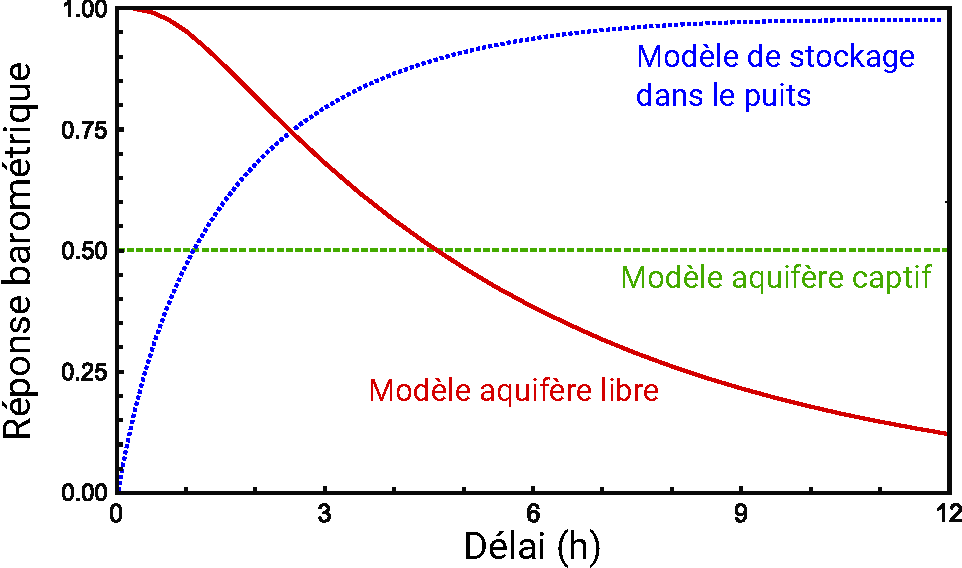
\includegraphics[width=\linewidth]{D113 Spane_2002.pdf}
  }
\end{tcbposter}

\end{document}